\subsubsection{Product Scanner}
The Product Scanner is found in the first tab in our HomeActivity. It was
implemented in the following manner:
\begin{description}
\item[Scan View] This was implemented as ScanFragment, a Fragment which holds a
Scan button which starts a new scan when pressed. The user chooses the store
they found the product at from a list on a Dialog and then the Barcode Scanner
application is launched using an Intent. An unsuccessful scan will bring up a
dialog asking the user whether they wish to try again. A successful scan brings
up a dialog which asks the user to update the product's price. The user is then
taken to BrowseFragment (described in the next section). An unsuccessful scan
takes the user to NewProductFragment.
\item[Store Creator] This was implemented as NewBranchFragment. The user is
asked to choose the store's franchise, location and city. If the city doesn't
exist as of yet the user must choose the province as well. The store is then
added to the server's datastore as well as the local database and the scan can
begin.
\item[Product Creator] This was implemented as NewProductFragment. The user is
asked to choose the product's name, brand, size and category . The product is
then added to the server's datastore as well as the local database and the user
is taken to the BrowseFragment.
\end{description} 
 \begin{figure}[h!]
\centering
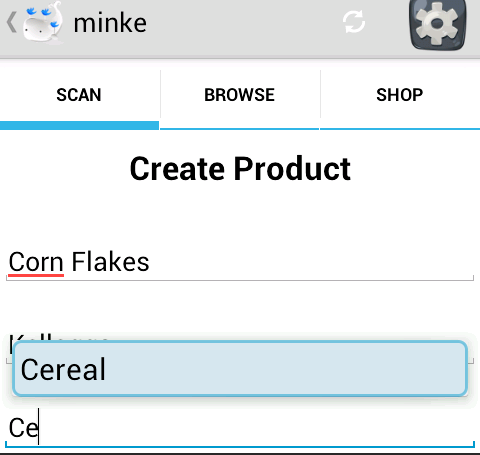
\includegraphics[width=0.3\textwidth]{new-product.png}
\caption{Product creation after a successful scan.}
\end{figure}
